\chapter{Resultados}\label{chapter:results}

A lo largo de esta tesis se han concebido y diseñado varios modelos para resolver la tarea de selección de respuestas a partir de un corpus previamente construido. En el presente capítulo, se expone un conjunto de experimentos desarrollados con el propósito de medir el desempeño de los modelos propuestos en dicha tarea.

\section{Medidas de Evaluación}

Con el propósito de medir la eficacia de los modelos propuestos es necesario la aplicación de medidas estándares utilizadas en el paradigma del aprendizaje automático. Para la evaluación de los modelos propuestos se utiliza como métrica la \textbf{Exactitud}. Asimismo, teniendo en cuenta el escenario también se utiliza como métrica de evaluación la puntuación característica de estos exámenes y que es la empleada realmente para calificar los exámenes cada año.

Supongamos que estamos en presencia de un problema de clasificación binario cualquiera, donde solo existen dos clases que llamaremos $C^{+}$ y $C^{-}$. Los posibles tipos de respuestas de un modelo se definen como:

\begin{description}
  \item \textbf{\textit{True Positive} (TP)}: Un ejemplo se clasifica en \textbf{TP}, traducido al español como Verdadero Positivo, cuando la clase predicha coincide con la clase correcta $C^{+}$. En este caso, la predicción hecha fue correcta.
  \item \textbf{\textit{False Positive} (FP)}: Un ejemplo se clasifica en \textbf{FP}, en español Falso Positivo, cuando el valor predicho es $C^{+}$, sin embargo su valor correcto es $C^{-}$. En este caso, el modelo hizo una predicción equivocada.
  \item \textbf{\textit{False Negative} (FN)}: Una instancia se clasifica en \textbf{FN}, en español Falso Negativo, cuando el valor predicho es $C^{-}$, sin embargo su clase correcta es $C^{+}$. En este caso, como en el anterior, el modelo hizo una predicción incorrecta.
  \item \textbf{\textit{True Negative} (TN)}: Una instancia se clasifica en \textbf{TN}, en español, Verdadero Negativo, cuando la clase predicha corresponde con la clase correcta $C^{-}$, lo que implica que el modelo hizo una predicción acertada.
\end{description}

Estos tipos de respuestas se representan visualmente en la matriz de confusión que se muestra en la tabla \ref{tab:confusion}.

\begin{table}[h!]
  \caption{Matriz de confusión para un problema de clasificación binario}
  \begin{center}
    \begin{tabular}{ccc|cc|cc}
        & Valor Correcto/Valor Predicho &    & $\mathbf{C}^{\boldsymbol{+}}$ & & $\mathbf{C}^{\boldsymbol{-}}$  \\
        \hline
        & $\mathbf{C}^{\boldsymbol{+}}$ &   & TP & & FN  \\
        \hline
        & $\mathbf{C}^{\boldsymbol{-}}$ &   & FP & & TN  \\
    \end{tabular}
  \end{center}
  \label{tab:confusion}
\end{table}

La \textbf{Exactitud} (en inglés \textit{Accuracy}) se interpreta como la razón entre las predicciones correctas ($TP + TN$) y la cantidad total de instancias que analizó el modelo. Se computa sobre los resultados generales del modelo y se define como:

\begin{equation}
  E = \frac{TP + TN}{\textit{Total de Ejemplos}}
\end{equation}

La métrica estándar para calificar este tipo de exámenes consiste en sumar tres puntos si la respuesta está correcta y -1 si es incorrecta.

\section{Técnicas de remuestreo}

En esta sección se detalla el proceso de entrenamiento de los modelos propuestos anteriormente. 

Dado que una instancia del conjunto original se convierte en varios ejemplos diferentes, una por cada posible respuesta y que solo una de las respuestas es correcta, el conjunto de datos resultante del procesamiento de texto es un conjunto desbalanceado. Por una instancia positiva pueden aparecer al menos 3 instancias negativas.

Un conjunto de datos desbalanceado es el problema en el que los datos que pertenecen a una clase son significativamente más altos o más bajos que los que pertenecen a otras clases, como es el caso. La mayoría de los algoritmos de clasificación ML/DL no están equipados para manejar clases desequilibradas y tienden a inclinarse hacia las clases mayoritarias.

Para enfrentar este problema se han implementado varias técnicas de remuestreo cuyo objetivo es equilibrar la cantidad de muestras en cada una de las clases. La idea más sencilla para balancear un conjunto de datos es añadiendo muestras de la clase minoritaria o eliminando de la clase mayoritaria, sin embargo, estás técnicas tienen riesgo de \textit{overfitting} y \textit{underfitting} respectivamente. En la práctica resultan más efectivas técnicas avanzadas como SMOTE (del inglés, \textit{Synthetic Minority Over-sampling Technique}) que crean datos sintéticos de la case minoritaria. Sin embargo, SMOTE no se desempeña bien en el ámbito de los datos textuales por la alta dimensionalidad de los vectores que se obtienen a partir de texto.

Teniendo en cuenta esto, se han implementado las siguientes técnicas de remuestreo:

\begin{itemize}
  \item \textit{Random Undersampling}: Este algoritmo consiste en eliminar del conjunto de datos transformados instancias negativas de manera aleatoria hasta igualar la cantidad de instancias positivas y negativas.
  \item \textit{Random oversampling}: Este proceso es muy similar al anterior desde el punto de vista de la aleatoriedad pero adiciona instancias positivas al \textit{dataset} hasta igualar la cantidad de instancias de cada etiqueta.
  \item \textit{Mixed oversampling}: El objetivo de esta técnica es reproducir el comportamiento de los algoritmos de generación sintética de datos. El concepto también es similar a \textit{Data Augmentation}, común en el procesamiento de imágenes, que implica la creación de nuevas instancias aplicando transformaciones (como rotar, trasladar, escalar, entre otras) las del conjunto de datos original. En este caso, para generar texto a partir de las oraciones originales se recurre a la traducción y al reemplazamiento por sinónimos. El algoritmo de traducción toma una oración y la traduce al idioma inglés, del inglés al alemán y luego, nuevamente al castellano. Se introduce un idioma intermedio para lograr una mayor diferencia entre la oración original y la resultante. Esto podría resultar contraproducente pues puede cambiar el sentido de la oración original, lo cual se verá en la evaluación de los modelos. Por otra parte, la otra técnica consiste en a partir de una oración obtener otra compuesta por las palabras más parecidas a cada una de las palabras de la oración original. Las palabras más similares a un témino dado se han determinado a partir del uso de sus \textit{word embeddings}. En este caso, se han utilizado \textit{embeddings} obtenidos aplicando el algoritmo Fasttext sobre el \textit{Spanish Billion Word Corpus}\footnote{http://crscardellino.github.io/SBWCE/} descargado de \cite{spanish-word-embeddings}. 
\end{itemize}

En las secciones posteriores se muestran los resultados de los modelos propuestos utilizando como entrenamiento las diferentes técnicas de remuestreo.

\section{Entrenamiento}

Además de los modelos de aprendizaje profundo detallados en el capítulo anterior, se implementa un modelo de regresión logística, que por su simplicidad, es utilizado como \textit{baseline} supervisado, al no existir soluciones anteriores que utilicen este tipo de aprendizaje.

La métrica utilizada por los autores del \textit{dataset} es la \textit{Exactitud} y la cantidad de puntos, ambos a nivel de examen. Lo que quiere decir que, aunque los enfoques supervisados implementados interpretan el problema como una tarea de clasificación binaria y se puede calcular la exactitud sobre el conjunto de datos transformado, no se utilizará esta forma para expresar los resultados finales en aras de poder comparar los resultados con los ya existentes en la literatura.

Por esta razón, esta sección se centra en el proceso de entrenamiento y el análisis de los resultados sobre el conjunto de datos transformado. Mientras que la próxima sección se centra en el cálculo de la \textbf{Exactitud} sobre los datos originales y presenta los resultados finales comparables con los ya existentes.

Para analizar el proceso de entrenamiento nos centraremos en estudiar la evolución de los algoritmos implementados sobre el conjunto de datos de entrenamiento resultante de aplicar la técnica de remuestreo \textit{Random Oversampling}. 

El objetivo de este análisis es comrpobar si la transformación a un problema de clasificación binario en este escenario es válida y si se corresponden con los resultados finales sobre el conjunto original.

En la Figura \ref{loss_lreg} se muestra la evolución de la función de pérdida durante el entrenamiento del modelo de Regresión Logística, mientras que en la Figura \ref{loss_all} del resto de los modelos supervisados, exceptuando el basado en BERT. Este último no se incluyó porque la cantidad de epochs utilizada es muy pequeña. La función de pérdida utilizada fue \textit{Binary Cross Entropy}.

\begin{figure}[!tb]
  \begin{center}
    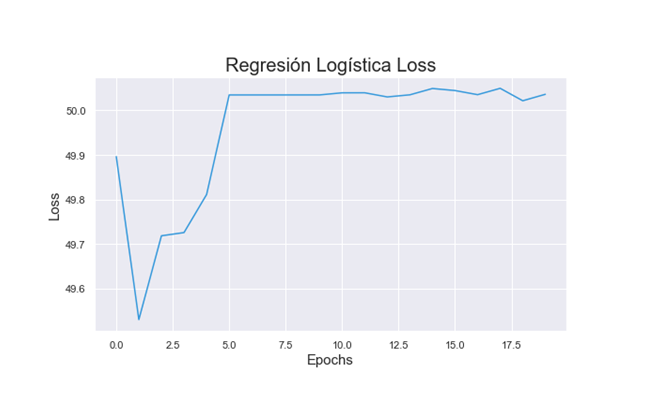
\includegraphics[angle=0, width=1\textwidth]{Graphics/loss_lreg.png}
  \end{center}
    \caption{Función de pérdida del modelo Regresión Logística durante el entrenamiento}\label{loss_lreg}
\end{figure}

\begin{figure}[!tb]
  \begin{center}
    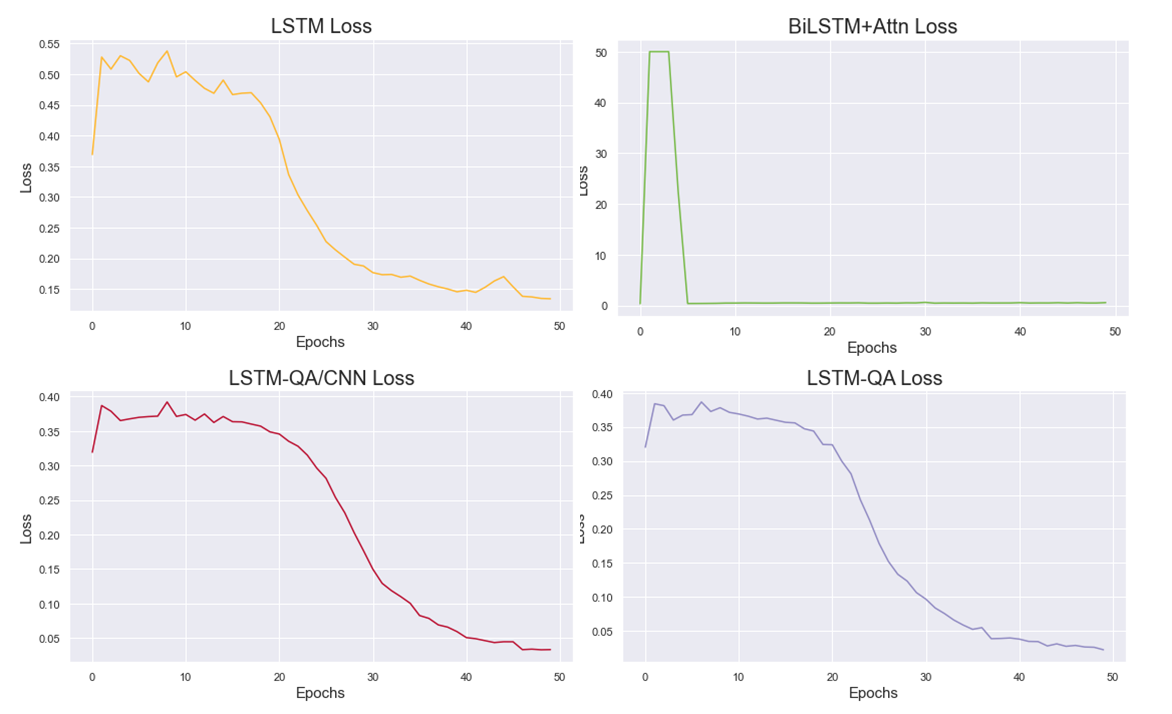
\includegraphics[angle=0, width=1\textwidth]{Graphics/loss_all.png}
  \end{center}
    \caption{Función de pérdida de los modelos supervisados durante el entrenamiento}\label{loss_all}
\end{figure}

Se puede observar que el modelo de regresión no logra minimizar la función de pérdida a partir de los datos de entrenamiento, por lo que se puede pensar que este modelo no tiene la capacidad o los datos de entrenamiento no son son suficientes, sufriendo de \textit{underfitting}. También se puede notar en la segunda imagen que el modelo BiLSTM+Attn aunque logra minimizar la pérdida, se queda por encima del resto de los modelos que logran minimizar a valores cercanos a 0,05. A partir del comportamiento de esta función, se espera que los modelos LSTM, LSTM-QA y LSTM-QA/CNN sean los que mejor desempeño alcancen.

En este caso, como estamos en presencia de conjuntos de datos imbalanceados, aunque se balanceó el de entrenamiento, el de validación y test no se modificaron en ese sentido, no es recomendable utilizar la exactitud como métrica de evaluación. Por esta razón, se visualiza la matriz de confusión para cada uno de los modelos entrenados.

En la Figura \ref{dev_cm} se muestra la matriz de confusión de los modelos sobre el conjunto de validación, mientras que la Figura \ref{test_cm} corresponde a los resultados sobre le conjunto de test.

\begin{figure}[!tb]
  \begin{center}
    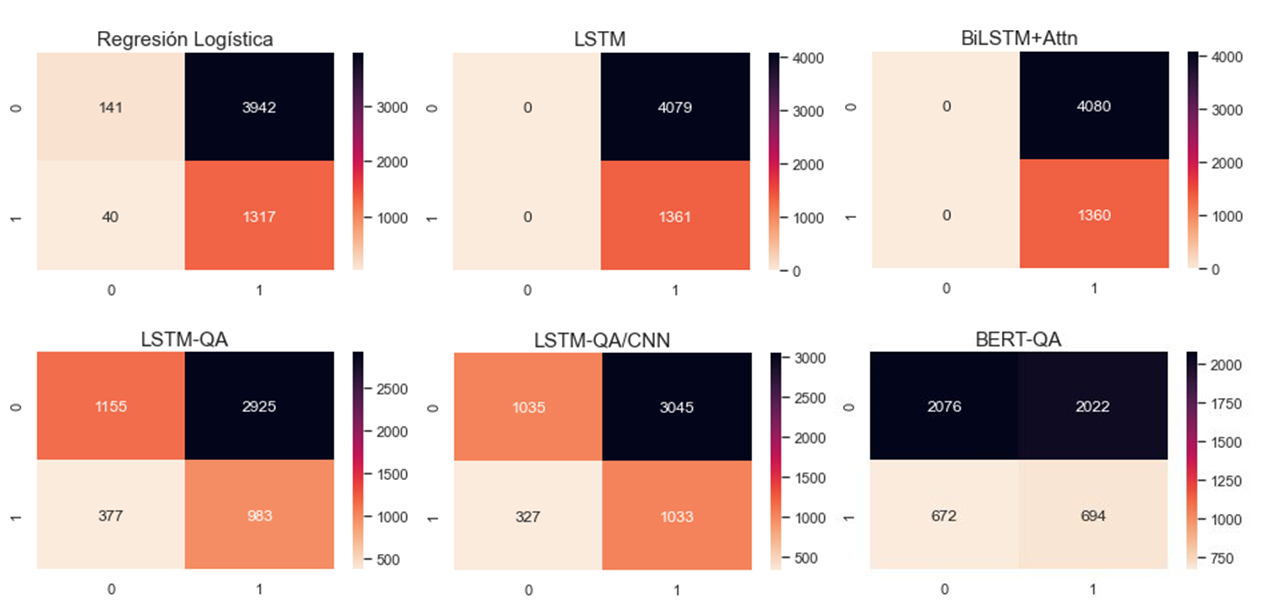
\includegraphics[angle=0, width=1\textwidth]{Graphics/dev_cm.png}
  \end{center}
    \caption{Matriz de confusión DEV}\label{dev_cm}
\end{figure}

\begin{figure}[!ht]
  \begin{center}
    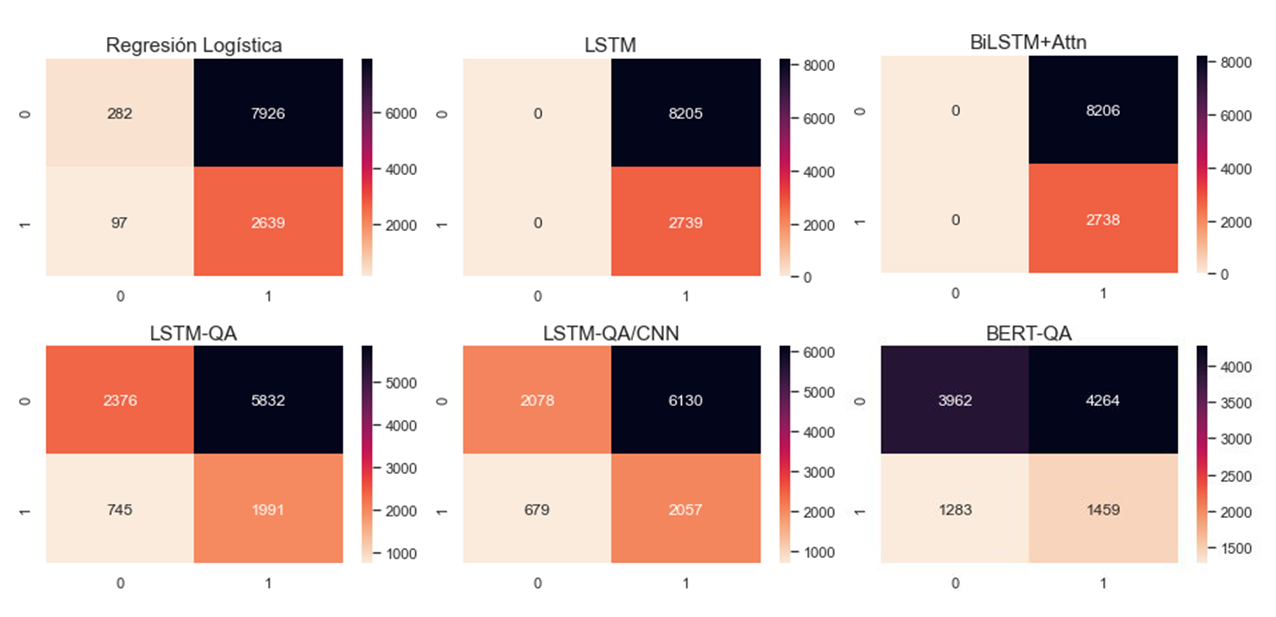
\includegraphics[angle=0, width=1\textwidth]{Graphics/test_cm.png}
  \end{center}
    \caption{Matriz de confusión TEST}\label{test_cm}
\end{figure}

En la Figura \ref{dev_cm} se puede notar como el algoritmo de regresión a pesar de no haber logrado optimizar la función de pérdida, da algunos resultados correctos. Por otra parte, es notable que LSTM y BiLSTM predicen siempre la clase positiva. Los últimos tres modelos son los que más han logrado aprender del conjunto de entrenamiento, sin embargo también se puede notar una tendencia a la clase positiva. Este comportamiento es muy similar en el conjunto de test como se puede observar en la Figura \ref{test_cm}. Predecir la clase postiva significa que los modelos dan una gran relevancia a la mayoría de las posibles respuestas. Sin embargo, esto necesariamente no tiene por qué ser negativo al ser aplicado en el problema original, pues en ese caso se toma como correcta solo la posible respuesta con mayor relevancia.

Tras este análisis se puede concluir que si bien algunos de los algoritmos han logrado aprender de los datos, especialmente los que incluyen el enfoque de recuperación de información, el desempeño no ha sido muy bueno de manera general, aunque era esperado dada los resultados tan bajos que se han obtenido también en la literatura. Esto puede tener varias causas: los algoritmos sufren de \textit{underfitting} y necesitan más entrenamiento sobre los mismos datos o necesitan más datos. El proceso de entrenamiento durante la experimentación se detuvo cuando se observó una estabilidad en la pérdida, por lo que existe una mayor posibilidad de que los datos no sean suficientes dada la complejidad del problema.

En la siguiente sección nos centraremos en exponer los resultados finales sobre el conjunto original.

\section{Evaluación}

Como se mencionó anteriormente, las preguntas del conjuntos de datos están separadas por categorías. Tras el análisis descriptivo inicial, se pudo notar que las palabrás más comunes al separar los datos diferían según la temática, o sea, el vocabulario varía de acuerdo al dominio. Por esta razón, se decide entrenar y evaluar los modelos tanto en el conjunto de datos completo, como en los subconjuntos resultantes de filtrar por materia.

La métrica utilizada por los autores del \textit{dataset} es la \textit{Exactitud} y la cantidad de puntos, ambos a nivel de examen. Lo que quiere decir que, aunque los enfoques supervisados implementados interpretan el problema como una tarea de clasificación binaria y se puede calcular la exactitud sobre el conjunto de datos transformado, no se utilizará esta forma en aras de poder comparar los resultados con los ya existentes en la literatura. 

De manera que, la métrica \textbf{Exactitud} no se computará sobre el conjunto transformado a binario, sino sobre los exámenes originales. Por lo tanto, una instancia se considera correcta si la pregunta como un todo fue respondida correctamente y no si cada una de las respuestas fueron clasificadas en positivo o negativo correctamente. La \textbf{Exactitud}, además, se considera adecuada ya que las clases en el problema actual (pregunta respondida correctamente o incorrectamente) tienen el mismo pero.

Dado que los modelos supervisados anteriores en su mayoría aplican la función sigmoide en la última capa, devuelven un número entre 0 y 1, que indica cuán relevante es la posible respuesta a la pregunta. Dada una pregunta del conjunto de datos original con sus posibles respuestas, cada par se transforma en una instancia vectorizada y se da como entrada al modelo de aprendizaje. La salida del modelo para cada una de las posibles respuestas es organizada y se elige como respuesta correcta la de mayor relevancia.

A continuación, se presentan los resultados alcanzados en este trabajo. Inicialmente se presentan los resultados alcanzados por categorías y posteriormente en el conjunto de datos general.

\subsection{Evaluación por categorías}

En esta sección, se analizan los resultados de aplicar las métricas antes mencionadas sobre el conjunto de evaluación obteniendo un conjunto de valores finales y concluyentes para cada modelo, de manera que se puedan comparar con los resultados actuales. El conjunto de validación está compuesto solamente por 6 exámenes, uno de cada categoría, mientras que el conjunto de evaluación está confomado por 12, 2 de cada rama.

En la Tabla \ref{comparison_points} se presentan los resultados obtenidos en función de la cantidad de puntos por todos los modelos implementados, teniendo en cuenta las categorías. Asimismo en la Tabla \ref{comparison_accuracy}, se comparan en función de la exactitud. Adicionalmente, en ambos casos, en las líneas inferiores se incluyen las métricas reportadas en \cite{2019-head-qa} sobre el conjunto de datos en español. 

Las columnas de la tabla corresponden al nombre del modelo, el método de remuestreo aplicado sobre el conjunto de entrenamiento y los nombre de los exámenes de acuerdo a la categoría: Biología (MIR), Enfermería (EIR), Farmacología (FIR), Medicina (MIR), Psicología (PIR) y Química (QIR). 

\begin{table}[!ht]
  \begin{center}
    \caption{Comparación de los modelos por categorías por Puntos}
    \begin{tabular}{l|c|c|c|c|c|c|c}
      \textbf{Modelo} & \textbf{Entrenamiento} & \textbf{BIR} & \textbf{EIR} & \textbf{FIR} & \textbf{MIR} & \textbf{PIR} & \textbf{QIR}\\
      \hline
      Regresión Logística & \textit{Oversampled} & -3 & 7 & -9 & \textcolor{red}{469} & -8 & -7 \\
      LSTM & \textit{Oversampled} & \textbf{43} & 23 & -17 & \textcolor{red}{320} & 9 & 51\\
      BiLSTM+Attn & \textit{Oversampled} & -22 & -6 & -37 & \textcolor{red}{342} & -8 & -9\\
      QA-LSTM & \textit{Oversampled} & 41 & 17 & -3 & -4 & 13 & -5\\
      QA-LSTM/CNN & \textit{Oversampled} & -2 & -16 & -1 & -18 & 17 & 21\\

      Regresión Logística & \textit{Mixed} & 3 & -6 & -9 & \textcolor{red}{461} & -8 & -13\\
      LSTM & \textit{Mixed} & 27 & 19 & \textbf{24} & \textcolor{red}{327} & -2 & -65\\
      BiLSTM+Attn & \textit{Mixed} & -3 & -6 & -13 & \textcolor{red}{323} & -8 & -9 \\
      QA-LSTM & \textit{Mixed} & 7 & 7 & -11 & 47 & -2 & -45 \\
      QA-LSTM/CNN & \textit{Mixed} & -15 & 1 & 6 & 35 & 29 & \textbf{51} \\

      QA-BERT & \textit{Undersampled} & 38 & \textbf{25} & 3 & 41 & \textbf{49} & -26 \\
      Sim-BERT & \textit{No} & -33 & -4 & -40 & 17 & -26 & 7 \\
      \hline
      RANDOM & - & -7 & 2.5 & -10,5 & -17,5 & 26,5 & 25 \\
      $BLIND_3$ & - & 9 & 44.5 & 19,5 & 22,5 & -1,5 & 25 \\
      $LENGTH$ & - & 67 & 70,5 & 47,5 & 18,5 & 50,5 & 47 \\
      $IR$ & - & 105 & 100,5 & 139,5 & 12,5 & 98,5 & 103,5 \\
    \end{tabular}
  \end{center}
  \label{comparison_points}
\end{table}

\begin{table}[!tb]
  \begin{center}
    \caption{Comparación de los modelos por categorías por Exactitud}
    \begin{tabular}{l|c|c|c|c|c|c|c}
      \textbf{Modelo} & \textbf{Entrenamiento} & \textbf{BIR} & \textbf{EIR} & \textbf{FIR} & \textbf{MIR} & \textbf{PIR} & \textbf{QIR}\\
      \hline

      Regresión Logística & \textit{Oversampled} & 0,25 & 0,26 & 0,24 & \textcolor{red}{0,76} & 0,24 & 0,24 \\
      LSTM & \textit{Oversampled} & \textbf{0,30} & \textbf{0,27} & 0,23 & \textcolor{red}{0,60} & 0,26 & \textbf{0,31}\\
      BiLSTM+Attn & \textit{Oversampled} & 0,23 & 0,24 & 0,21 & \textcolor{red}{0,62} & 0,24 & 0,24\\
      QA-LSTM & \textit{Oversampled} & 0,25 & \textbf{0,27} & 0,25 & 0,24 & 0,26 & 0,24\\
      QA-LSTM/CNN & \textit{Oversampled} & 0,29 & 0,23 & 0,25 & 0,23 & 0,27 & 0,27\\

      Regresión Logística & \textit{Mixed} & 0,25 & 0,24 & 0,24 & \textcolor{red}{0,76} & 0,24 & 0,23\\
      LSTM & \textit{Mixed} & 0,28 & \textbf{0,27} & \textbf{0,28} & \textcolor{red}{0,60} & 0,25 & 0,32\\
      BiLSTM+Attn & \textit{Mixed} & 0,25 & 0,24 & 0,24 & \textcolor{red}{0,60} & 0,24 & 0,24 \\
      QA-LSTM & \textit{Mixed} & 0,26 & \textbf{0,27} & 0,24 & 0,30 & 0,25 & 0,20 \\
      QA-LSTM/CNN & \textit{Mixed} & 0,23 & 0,25 & 0,26 & 0,29 & 0,28 & \textbf{0,31} \\

      QA-BERT & \textit{Undersampled} & 0,27 & 0,26 & 0,25 & 0,27 & \textbf{0,28} & 0,24\\
      Sim-BERT & \textit{No} & 0,21 & 0,25 & 0,21 & 0,27 & 0,22 & 0,26\\
      \hline
      $RANDOM$ & - & 0,24 & 0,25 & 0,24 & 0,23 & 0,28 & 0,28 \\
      $BLIND_3$ & - & 0,26 & 0,29 & 0,27 & 0,27 & 0,24 & 0,27 \\
      $LENGTH$ & - & 0,32 & 0,32 & 0,30 & 0,27 & 0,30 & 0,30 \\
      $IR$ & - & 0,36 & 0,36 & 0,40 & 0,26 & 0,36 & 0,36 \\

    \end{tabular}
  \end{center}
  \label{comparison_accuracy}
\end{table}

Los modelos incluidos en la parte inferior de la tabla consisten en:
\begin{itemize}
  \item $RANDOM$: Seleccionar una respuesta de manera aleatoria.
  \item $BLIND_3$: Seleccionar siempre la tercera opción.
  \item $LENGTH$: Seleccionar la respuesta más larga.
  \item $IR$: Modelo de RI implementado en \cite{2019-head-qa} que utiliza como corpus artículos de Wikipedia.
\end{itemize}

Al analizar los resultados obtenidos en función de la cantidad de puntos, se puede notar que los algoritmos supervisados si bien alcanzan resultados superiores al modelo aleatorio la mayoría de ellos, no superan al modelo basado en recuperación de información. Los modelos que más baja puntuación alcanzan son el de regresión logística y el modelo no supervisado construido sobre BERT.
Tras el análisis anterior de los modelos durante la etapa de entrenamiento, el comportamiento del regresor era esperado. Por otra parte, el fallo del modelo BERT-SIM reafirma que un simple \textit{matching} o coincidencia entre las palabras de la pregunta y la respuesta no es suficientes para resolver este problema.

Los resultados en función de exactitud reflejan un comportamiento muy similar. Los modelos que mejor desempeño han alcanzado son el LSTM, QA-LSTM y QA-BERT.

\subsection{Evaluación general}

En esta sección se exponen los resultados tras entrenar y evaluar los modelos sobre todo el conjunto de datos, sin tener en cuenta las materias de cada pregunta. En este caso, solamente se exponen los resultados alcanzados por nuestros modelos, pues en el artículo \cite{2019-head-qa} no se desarrollaron modelos siguiendo este enfoque. 

En la Tabla \ref{comparison_points_general} se presentan los resultados obtenidos en función de la cantidad de puntos por todos los modelos implementados. De manera análoga, en la Tabla \ref{comparison_acc_general} se muestra en función de la exactitud. En cada caso se muestras las puntuaciones media y máximas obtenidas.

\begin{table}[!tb]
  \begin{center}
    \caption{Comparación general por cantidad de puntos TEST}
    \begin{tabular}{l|c|c|c}
      \textbf{Modelo} & \textbf{Entrenamiento} & \textbf{Media Pts.} & \textbf{Max Pts.}\\
      \hline
      Regresión Logística & Desbalanceado & -8 & 29 \\
      LSTM & Desbalanceado & 1 & 37 \\
      BiLSTM+Attn & Desbalanceado & 15 & 93 \\
      QA-LSTM & Desbalanceado & 15 & 74 \\
      QA-LSTM/CNN & Desbalanceado & 11 & 36 \\

      Regresión Logística & \textit{Oversampled} & -5 & 37 \\
      LSTM & \textit{Oversampled} & 2 & 56 \\
      BiLSTM+Attn & \textit{Oversampled} & -2 & 21 \\
      QA-LSTM & \textit{Oversampled} & 9 & 45 \\
      QA-LSTM/CNN & \textit{Oversampled} & 7 & 61 \\

      Regresión Logística & \textit{Mixed} & -9 & 21 \\
      LSTM & \textit{Mixed} & 11 & 39 \\
      BiLSTM+Attn & \textit{Mixed} & -3 & 40 \\
      QA-LSTM & \textit{Mixed} & \textbf{23} & \textbf{101} \\
      QA-LSTM/CNN & \textit{Mixed} & 4 & 49 \\

      QA-BERT & \textit{Undersampled} & 3 & 41 \\
      Sim-BERT & \textit{No} & -13 & 29 \\
    \end{tabular}
  \end{center}
  \label{comparison_points_general}
\end{table}

\begin{table}[!tb]
  \begin{center}
    \caption{Comparación general por cantidad de Exactitud TEST}
    \begin{tabular}{l|c|c|c}
      \textbf{Modelo} & \textbf{Entrenamiento} & \textbf{Media Exact.} & \textbf{Max Exact.}\\
      \hline
      Regresión Logística & Desbalanceado & 0, 24 & 0,28\\
      LSTM & Desbalanceado & 0,25 & 0,29 \\
      BiLSTM+Attn & Desbalanceado & \textbf{0,27} & \textbf{0,35} \\
      QA-LSTM & Desbalanceado & 0,26 & 0,33 \\
      QA-LSTM/CNN & Desbalanceado & 0,26 & 0,29 \\

      Regresión Logística & \textit{Oversampled} & 0.24 & 0,29 \\
      LSTM & \textit{Oversampled} & 0,25 & 0,31 \\
      BiLSTM+Attn & \textit{Oversampled} & 0,25 & 0,27 \\
      QA-LSTM & \textit{Oversampled} & 0,26 & 0,30 \\
      QA-LSTM/CNN & \textit{Oversampled} & 0,26 & 0,32 \\

      Regresión Logística & \textit{Mixed} & 0,24 & 0,27 \\
      LSTM & \textit{Mixed} & 0,26 & 0,29 \\
      BiLSTM+Attn & \textit{Mixed} & 0,25 & 0,29 \\
      QA-LSTM & \textit{Mixed} & \textbf{0,27} & \textbf{0,36} \\
      QA-LSTM/CNN & \textit{Mixed} & 0,25 & 0,30 \\

      QA-BERT & \textit{Undersampled} & 0,25 & 0,30 \\
      Sim-BERT & \textit{No} & 0,23 & 0,28 \\
      
    \end{tabular}
  \end{center}
  \label{comparison_acc_general}
\end{table}

Nuevamente los modelos que menor desempeño muestran son el regresor logístico y BERT-SIM. Mientras que el que mayor puntuación alcanza es LSTM-QA cuando fue entrenado con el conjunto balanceado empleando el algoritmo \textit{Mixed Oversampling}. Se puede notar que la media de las puntuaciones al entrenar con todos los datos es muy similar a la alcanzada por los modelos independientes. Mientras que la puntuación máxima en algunos casos muestra un incremento.

Sin embargo, se debe tener en cuenta que el conjunto de datos de evaluación consta de 12 exámenes distribuidos en las 6 categorías y el de validación, con solo 6. Por esta razón, no se considera que este \textit{dataset} esté preparado aún para ser utilizado por algoritmos supervisados. Si bien es cierto que la cantidad de preguntas es grande, la probabilidad de que una pregunta se parezca a preguntas de años anteriores es baja cuando solo se cuenta con un histórico de alrededor de 5 años, teniendo en cuenta que cada examen tiene entre 200 y 250 preguntas y que los exámenes están separados por categorías.

De manera general, se puede afirmar que no hay grandes diferencias en los resultados en función de los datos de entrenamiento y las técnicas de remuestreo utilizadas. 

Los algoritmos de clasificación, a diferencia de los algoritmos de regresión, durante el entrenamiento minimizan una función de pérdida seleccionada y no directamente, la exactitud de los modelos, aunque ambas estén relaciondas. De manera que, el desempeño de un modelo, depende en gran medida de la función de pérdida seleccionada. La autora considera que una función de pérdida diseñada para maximizar la importancia de una respuesta correcta y penalizar una incorrecta podrá ofrecer notables ventajas y mejorar el desempeño de los algoritmos supervisados. 

\section{Discusión de los resultados}

Tras el análisis de los resultados se puede afirmar que el conocimiento adquirido por los modelos durante la etapa de entrenamiento es válido y puede ser utilizado para la selección de respuestas. Los modelos supervisados no mostraron un desempeño superior a los modelos del estado del arte sobre este conjunto de datos, pero tampoco obtuvieron resultados muy por debajo. Sin embargo y aunque los resultados son comparables con los modelos previamente existentes, continúan estando muy lejos de las puntuaciones alcanzadas por humanos. Teniendo en cuenta que en el año 2016 la media de las 10 mejores notas según \cite{2019-head-qa} está alrededor de los 600 puntos y las notas de corte cercanas a los 200, los modelos automáticos aún están lejos de resolver este problema.

Los modelos han demostrado que no tienen la capacidad de resolver este problema sobre este conjunto de datos. Dada la complejidad del problema en cuestión, la cantidad de datos no es suficiente para construir un modelo robusto basado solamente en aprendizaje supervisado. 